Nel panorama contemporaneo, l'Information Retrieval (IR) è soggetto a un continuo processo di innovazione, spinto dalla rapida evoluzione delle tecnologie dell'informazione e dalle crescenti esigenze informative della società. L'IR sta affrontando sfide sempre più complesse, ma sta anche beneficiando di approcci e tecniche avanzate che stanno ridefinendo il modo in cui le informazioni vengono recuperate, elaborate e presentate agli utenti. Questa sezione esamina lo stato attuale dell'Information Retrieval, evidenziando le tendenze chiave e le tecnologie emergenti che stanno plasmando il campo.

\subsubsection{Approcci Basati su Apprendimento Automatico e Intelligenza Artificiale}
Un'evoluzione significativa nell'IR è l'ampio utilizzo dell'apprendimento automatico e dell'intelligenza artificiale per migliorare la precisione e la personalizzazione dei risultati di ricerca. Gli algoritmi di machine learning vengono addestrati su grandi insiemi di dati per comprendere le intenzioni degli utenti e valutare la rilevanza dei documenti. L'adozione di modelli neurali e reti neurali profonde (deep learning) ha portato a miglioramenti nella comprensione del linguaggio naturale e nella capacità di interpretare le query in modo più accurato.
All'interno della figura~\ref{fig:typesofmodel} sono riportati i tipi di modelli di Information Retrieval. È inoltre indicata anche la tipologia di approccio utilizzato per la costruzione del modello, le sue basi matematiche e anche alcune caratteristiche come l'utilizzo o meno della interdipendenza tra i termini, ossia quanto un termine può influire sul prossimo.

\begin{center}
    \begin{figure}[H]
        \centering
        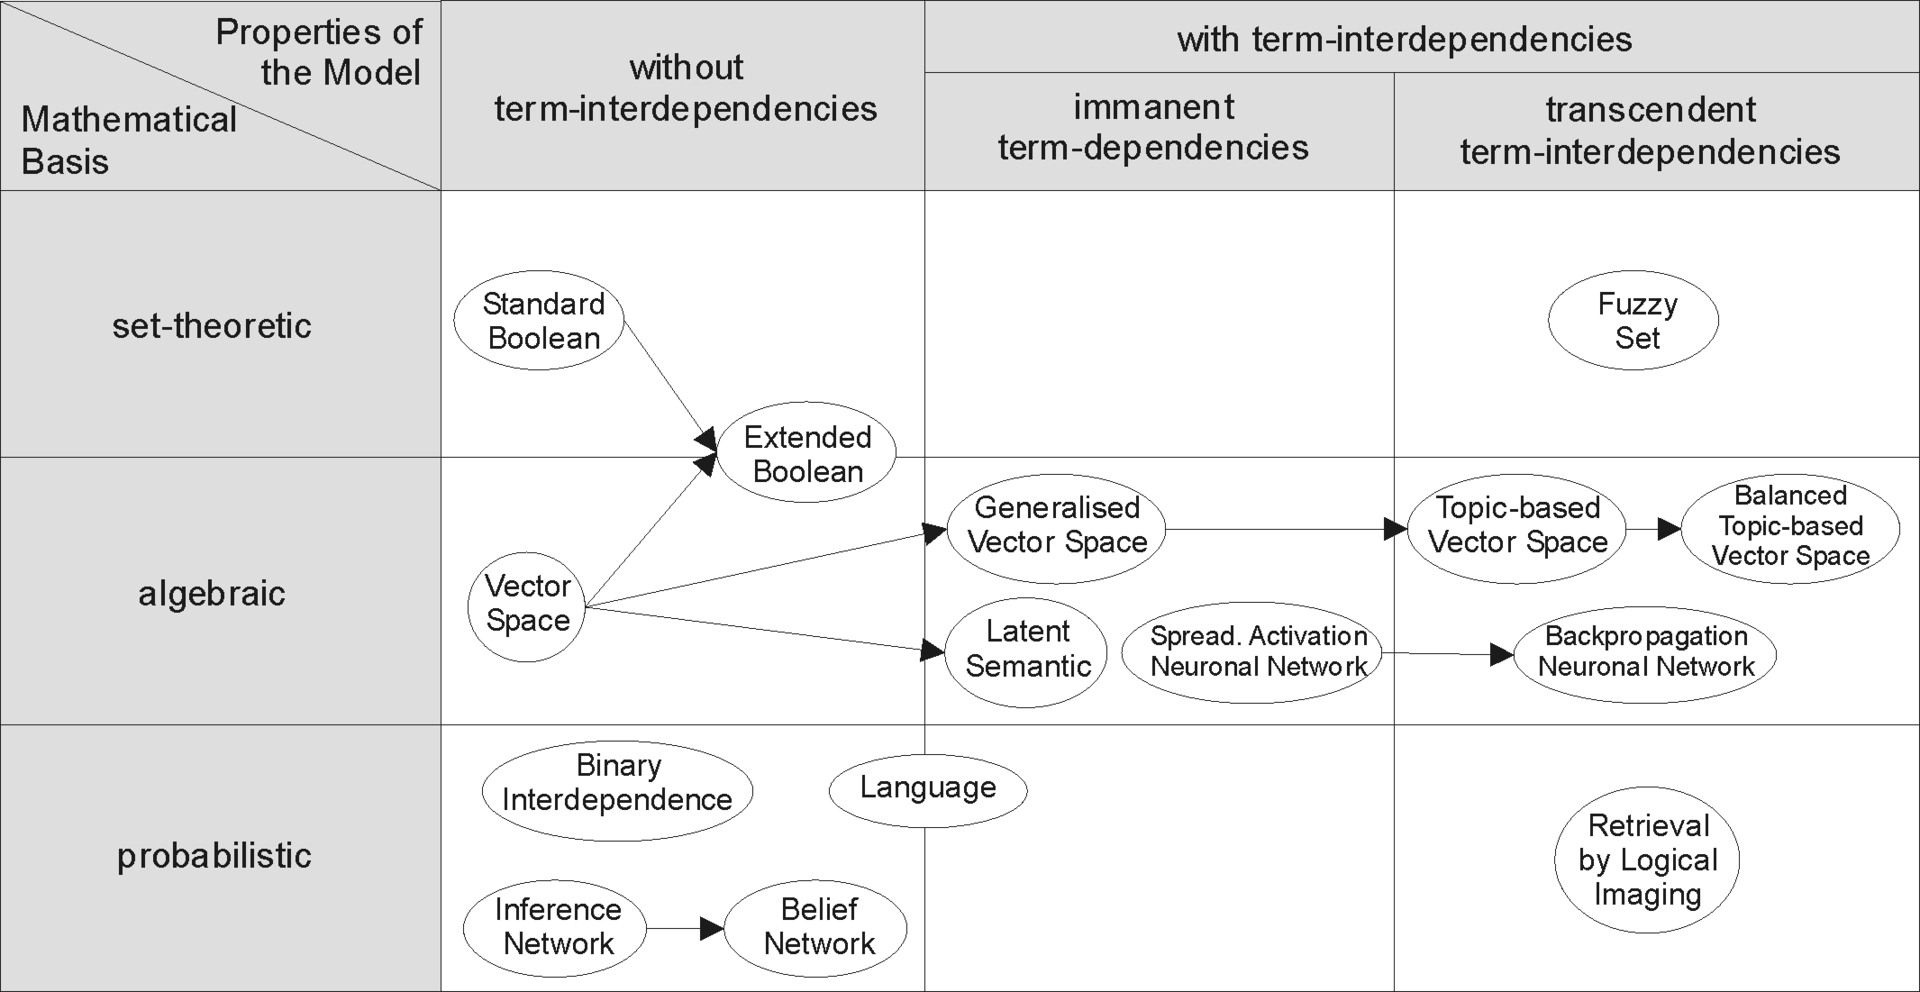
\includegraphics{images/typesofmodel.png}
        \caption{Tipi di modelli di Information Retrieval}
        \label{fig:typesofmodel}
    \end{figure}
\end{center}

\subsubsection{Ricerca Conversazionale e Interazione Uomo-Macchina}
L'IR sta sempre più abbracciando la ricerca conversazionale e l'interazione uomo-macchina. L'uso di assistenti vocali e chatbot basati su IR consente agli utenti di porre domande e ottenere risposte in modo più naturale e intuitivo. Questo richiede la comprensione di contesto, ambiguità e sfumature nelle query, oltre a fornire risposte coerenti e pertinenti.

\subsubsection{Ricerca Multimodale}
Con la crescente disponibilità di contenuti multimediali come immagini e video, l'IR si sta estendendo alla ricerca multimodale. Questo richiede l'elaborazione e l'integrazione di dati di diversi tipi, come testo, immagini e audio, per fornire risultati che riflettano la diversità dei contenuti presenti nelle collezioni digitali.

\subsubsection{Personalizzazione e Contestualizzazione}
L'IR sta diventando sempre più personalizzato, adattandosi alle preferenze e alle esigenze degli utenti individuali. I sistemi di raccomandazione basati su IR analizzano il comportamento passato dell'utente e forniscono risultati che sono più rilevanti e pertinenti per loro. Inoltre, la contestualizzazione sta guadagnando importanza, poiché i sistemi di IR cercano di comprendere il contesto in cui viene posta una query al fine di offrire risultati più precisi e utili.

\subsubsection{Etica, Privacy e Bias}
Con l'aumento dell'uso dell'IR, emergono preoccupazioni legate all'etica, alla privacy e ai bias. La personalizzazione e la profilazione degli utenti sollevano questioni sulla privacy e sulla gestione dei dati personali. Inoltre, l'IR deve affrontare il rischio di introdurre o amplificare bias culturali, politici o di genere nei risultati di ricerca, il che richiede un'attenzione crescente alla giustizia e all'equità nei sistemi di recupero dell'informazione.

In conclusione, lo stato dell'arte dell'Information Retrieval è caratterizzato da una fusione di approcci tradizionali e nuove tecnologie avanzate. L'adozione dell'apprendimento automatico, dell'intelligenza artificiale e la comprensione del contesto stanno ridefinendo l'esperienza di ricerca e recupero delle informazioni. Tuttavia, l'IR affronta anche sfide legate all'etica, alla privacy e all'equità, che richiedono attenzione continua. L'Information Retrieval rimane un campo dinamico e in evoluzione, destinato a plasmare ulteriormente il modo in cui le persone interagiscono con le informazioni nel mondo digitale in continua crescita.
